Esta seção apresenta as principais telas do sistema Web desenvolvidas em Node.js
(Express + Sequelize) com MySQL e EJS. Esta versão não possui todas as funcionalidades
finais, mas demonstra a estrutura básica e a navegação entre as páginas, além do funcionamento
do banco de dados.
\medskip

\begin{figure}[H]
\centering
\caption{Interface Web - Tela de Login}
\label{fig:interface-web-tela-login}
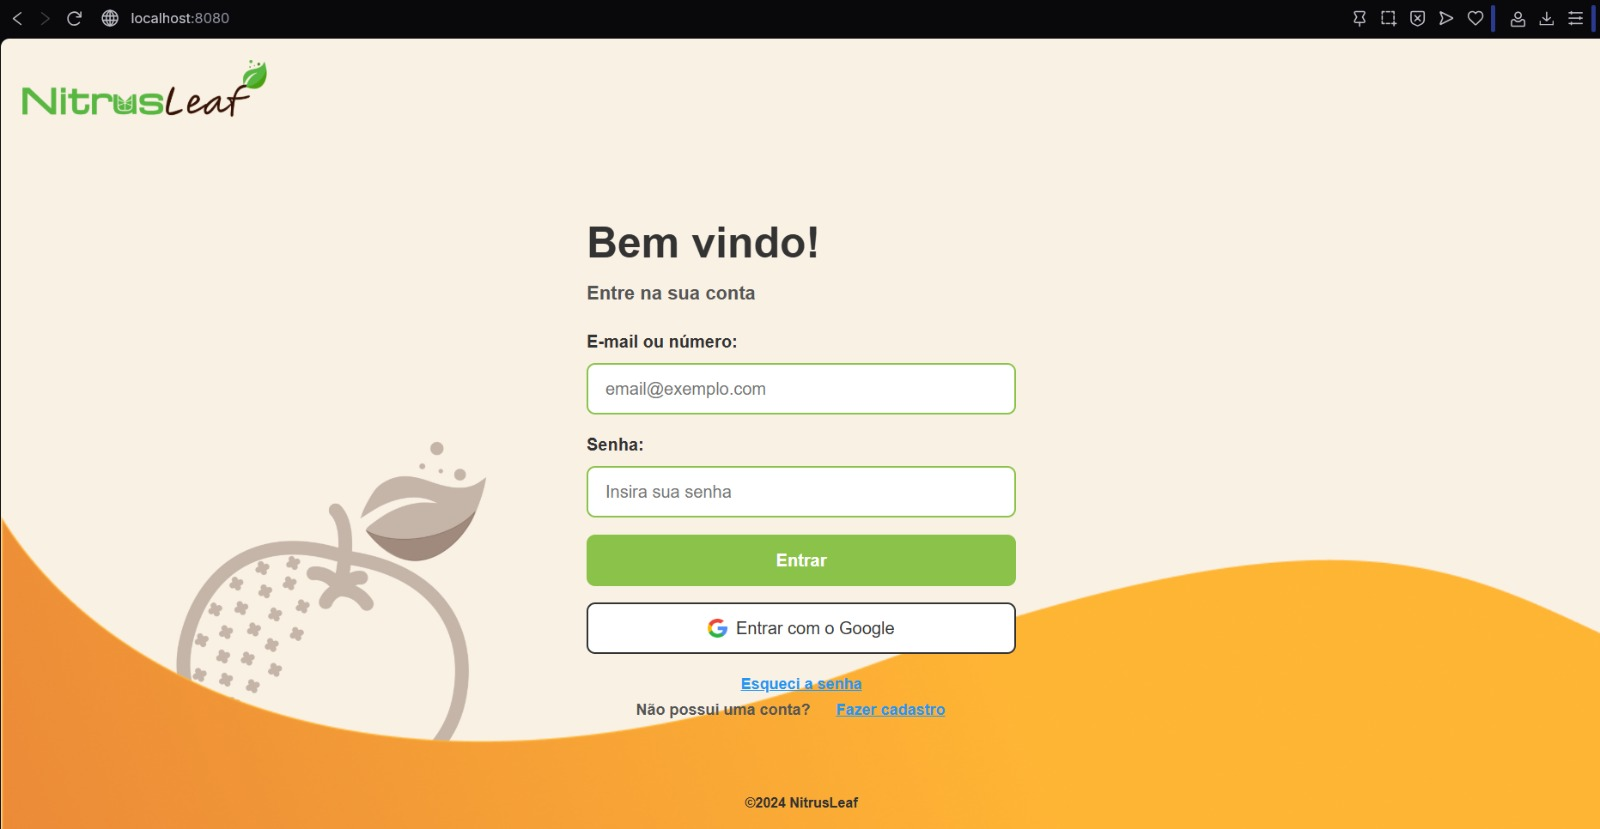
\includegraphics[width=0.8\textwidth]{Images/AppLogin.png}
\SourceOrNote{Equipe 21 - Vitalliz (2025)}
\end{figure}

A tela de login está fiel ao protótipo, com margem para 
ajustes futuros de UX/UI. A autenticação foi implementada via middleware, 
reforçando a segurança.

\begin{figure}[H]
\centering
\caption{Interface Web - Tela de Início}
\label{fig:interface-web-tela-inicio}
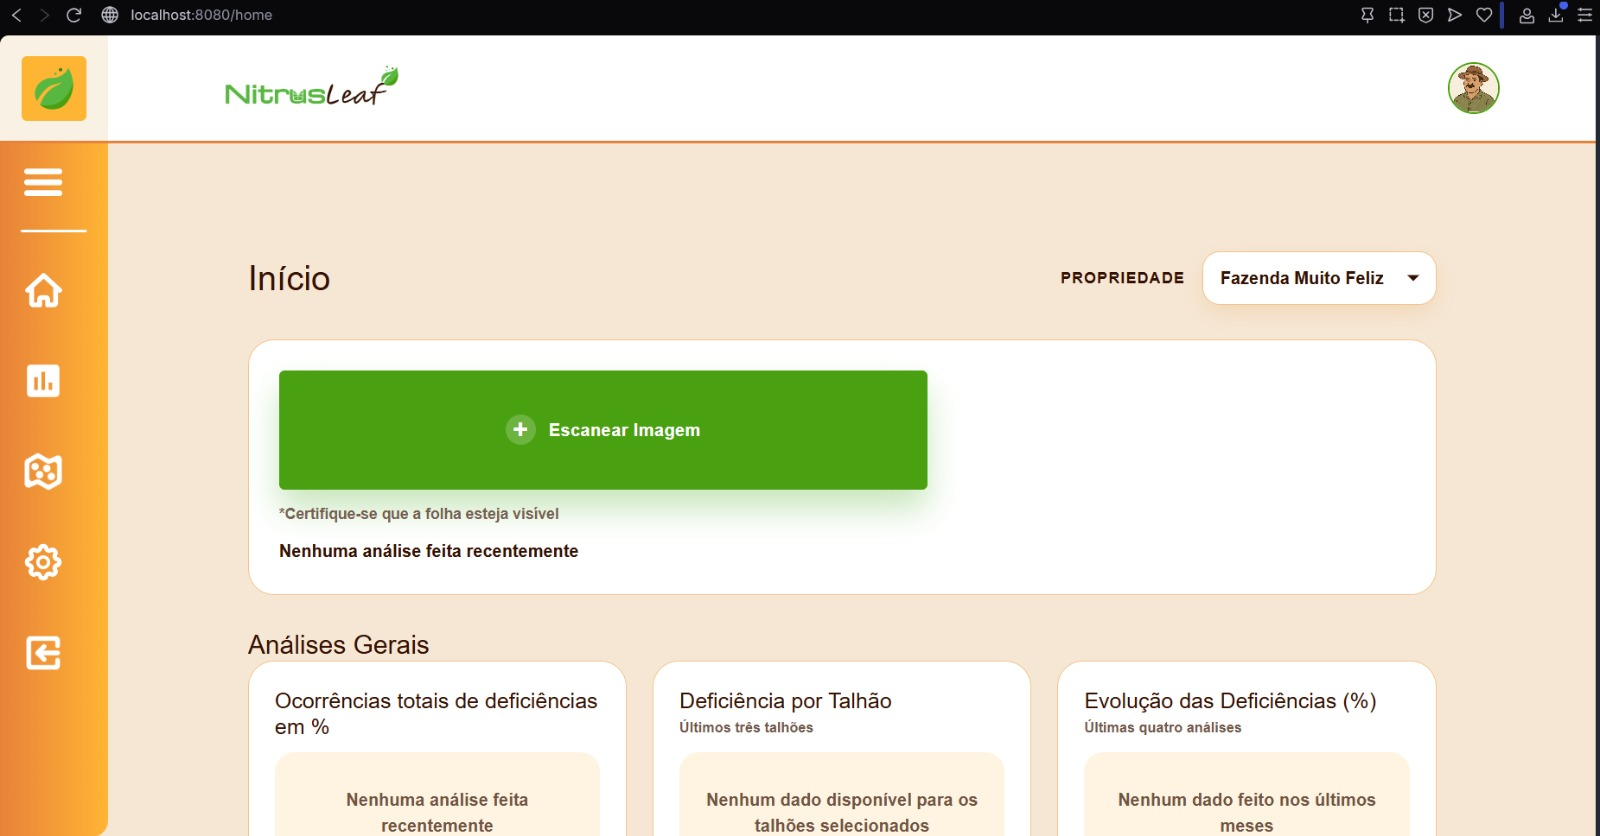
\includegraphics[width=0.8\textwidth]{Images/AppInicio.jpeg}
\SourceOrNote{Equipe 21 - Vitalliz (2025)}
\end{figure}

A tela de início é a primeira tela que o usuário vê após fazer login no sistema. 

\medskip

\begin{figure}[H]
\centering
\caption{Interface Web - Tela de Resultados}
\label{fig:interface-web-tela-resultados}
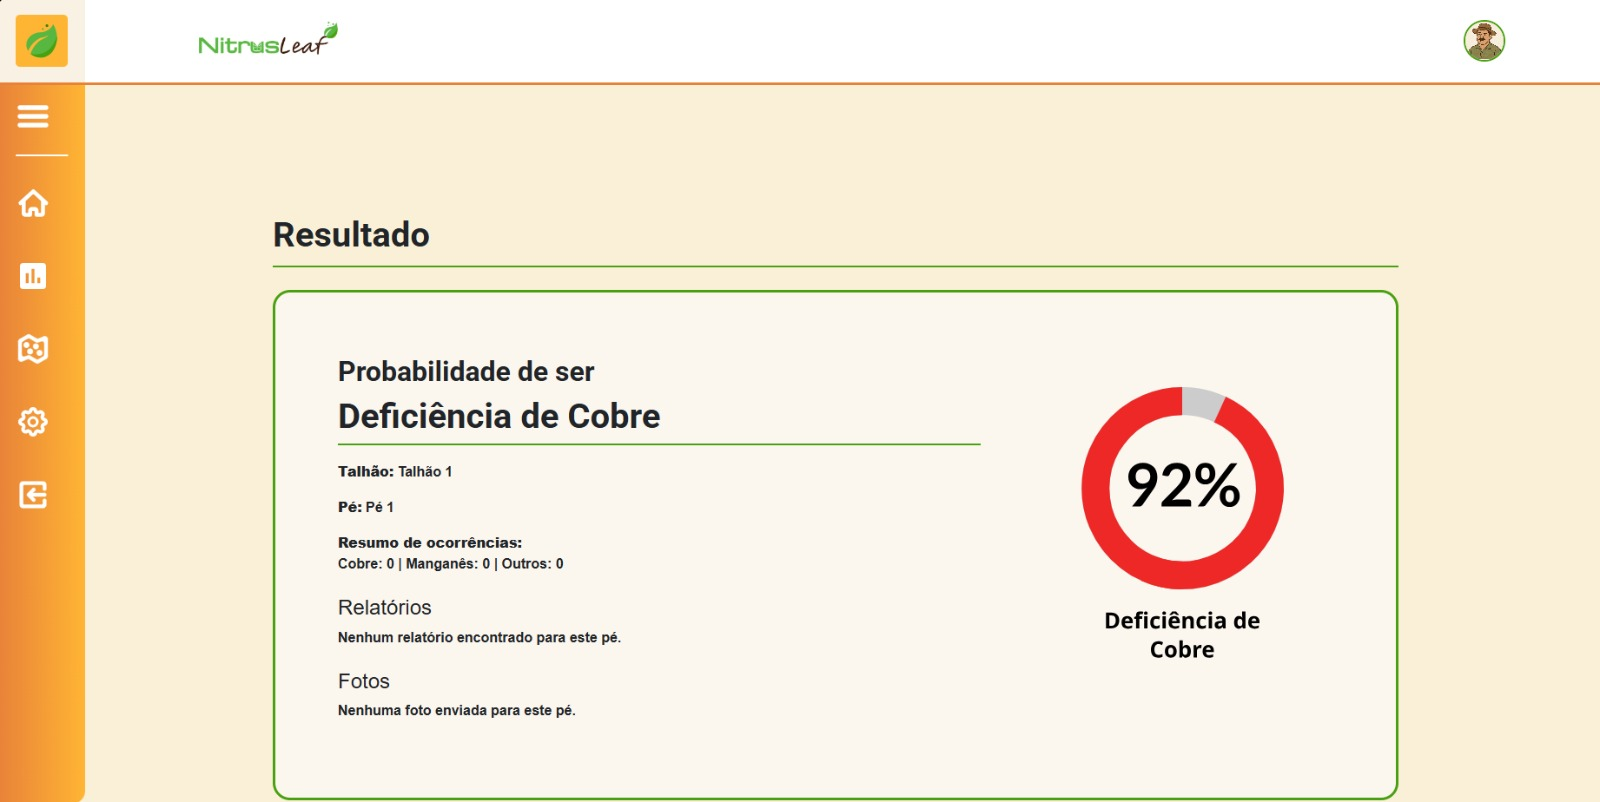
\includegraphics[width=0.8\textwidth]{Images/AppResultado.jpeg}
\SourceOrNote{Equipe 21 - Vitalliz (2025)}
\end{figure}

A tela de Resultados exibe os resultados detalhados das análises realizadas na
imagem enviada, permitindo melhor visualização do diagnóstico.
\medskip

\begin{figure}[H]
\centering
\caption{Interface Web - Tela de Histórico}
\label{fig:interface-web-tela-historico}
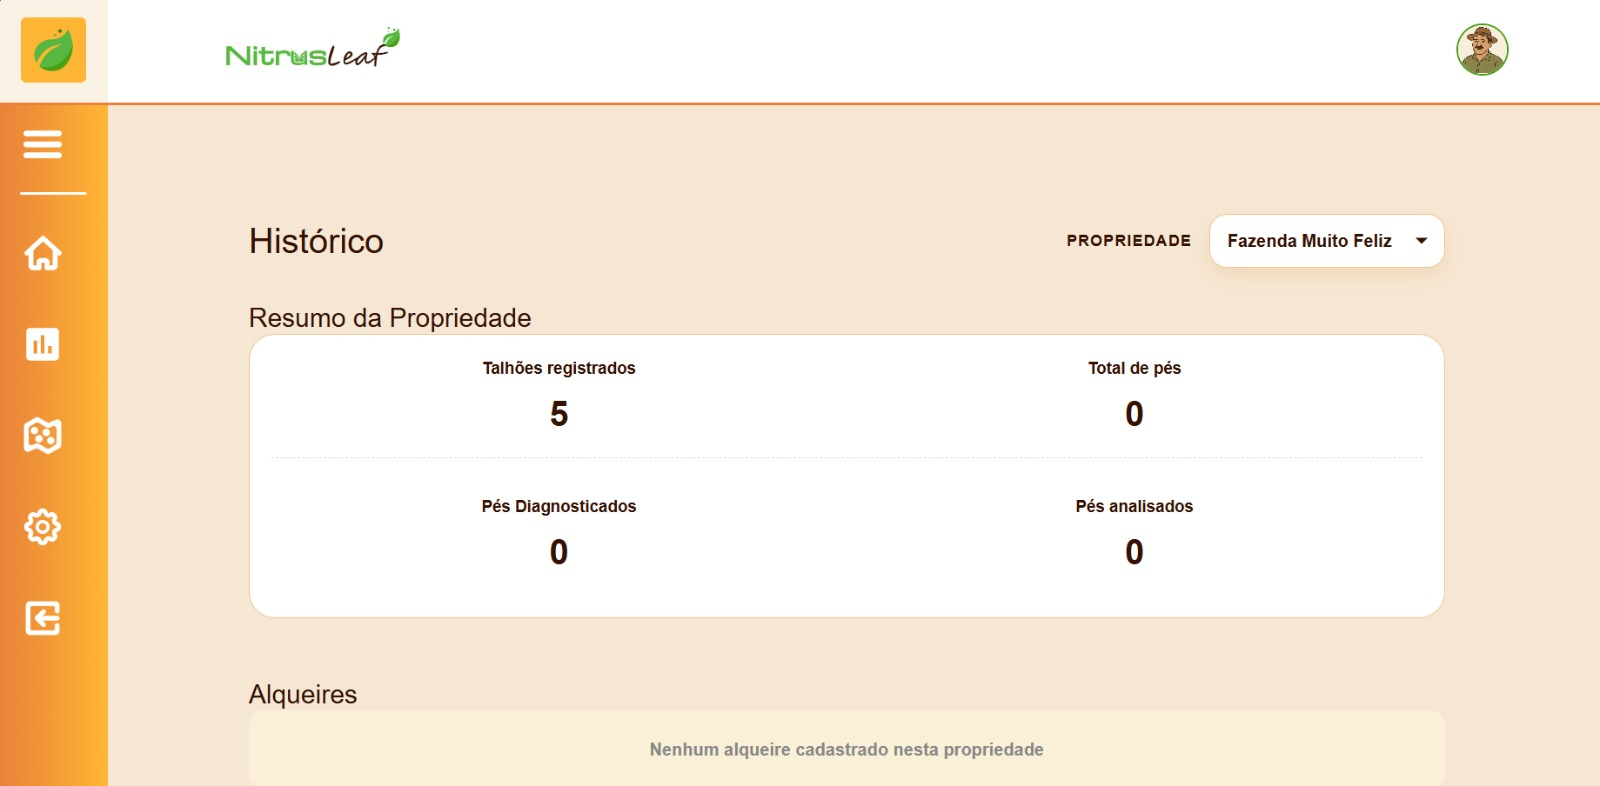
\includegraphics[width=0.8\textwidth]{Images/AppHistorico.jpeg}
\SourceOrNote{Equipe 21 - Vitalliz (2025)}
\end{figure}

A tela de histórico permite que o usuário visualize suas interações anteriores com o sistema, 
facilitando o acompanhamento de suas atividades e resultados ao longo do tempo.
\medskip


\begin{figure}[H]
\centering
\caption{Interface Web - Tela de Mapa}
\label{fig:interface-web-tela-mapa}
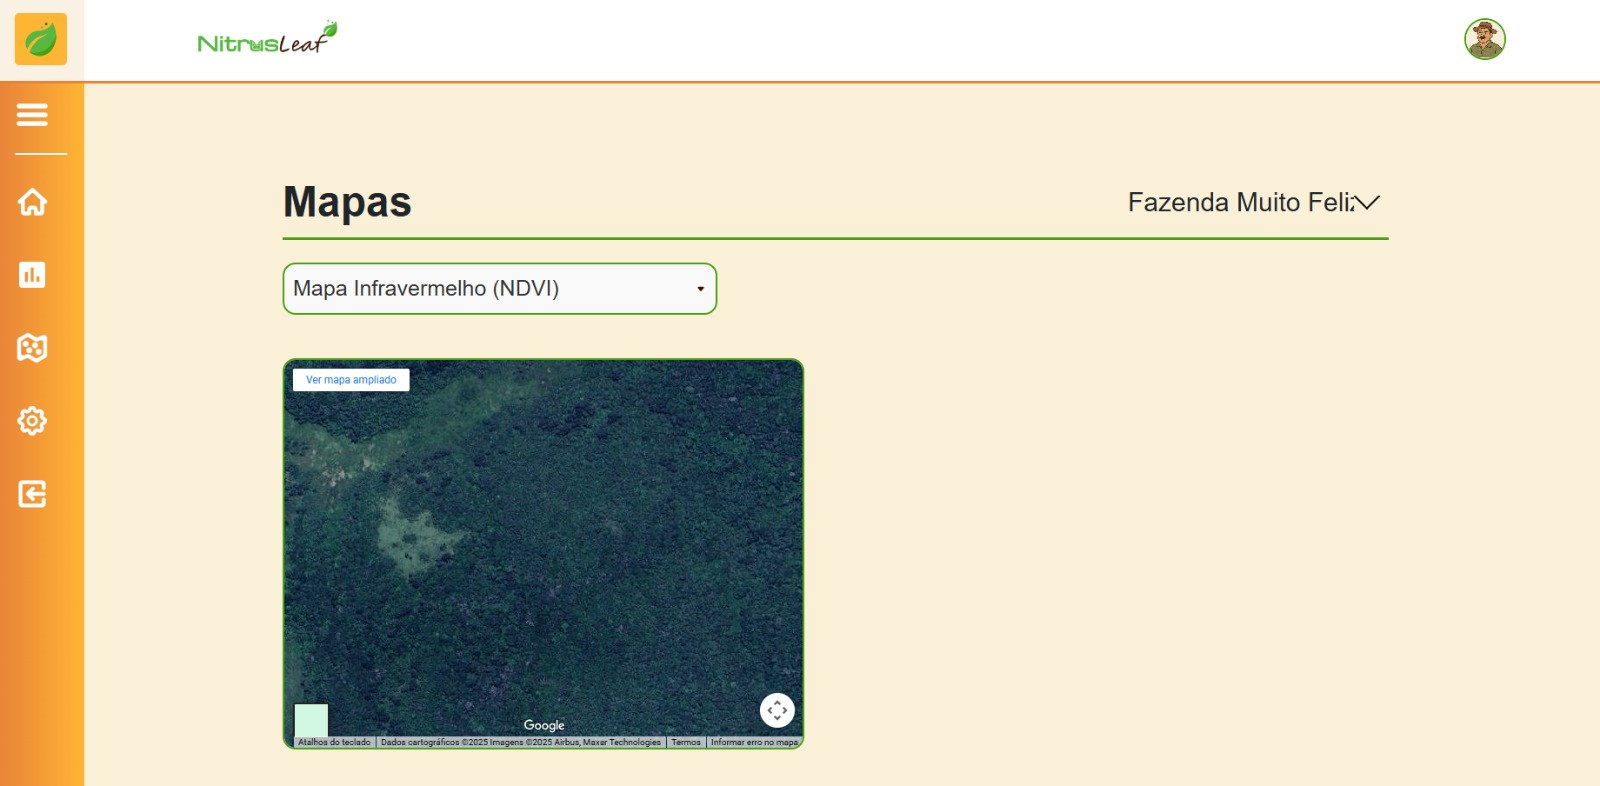
\includegraphics[width=0.8\textwidth]{Images/AppMapa.jpeg}
\SourceOrNote{Equipe 21 - Vitalliz (2025)}
\end{figure}

A tela de mapa permite que o usuário visualize a localização geográfica da propriedade.
\medskip
